\documentclass[10pt,a4paper]{book}
\usepackage[utf8]{inputenc}
\usepackage[english]{babel}
\usepackage{amsmath}
\usepackage{amsfonts}
\usepackage{amssymb}
\usepackage{wrapfig}
\usepackage{mathtools}
\usepackage{graphicx}
\usepackage{cancel}
\usepackage[left=2cm,right=2cm,top=2cm,bottom=2cm]{geometry}
\usepackage{physics}
\usepackage{multicol}
\usepackage{caption}
\usepackage{subcaption}
\author{Alessandro Pacco}
\title{DM-MMC, 2020}
\begin{document}
\maketitle


\section*{De la forme des arbres}

%It is reasonable to suppose that all the trees will try to become as tall as possible until they reach a point after which they would not be in a balanced position and they would break. Therefore our problem is similar to the problem encountered in class regarding the "obélisque de la concorde", in which we need to compute at what height there is a high 88risk of rupture. We will denote by $d$ the diameter of the trunck of the tree and by $E$ the Young modulus of the tree (if we assume the tree to be a uniform cylinder). 
%
%Then  denoting by $\rho$ the radius of curvature of the line  that links all the successive centers of the circles building the cylinder. Theory of elasticity given in class tells us that:
%\[
%M = E I \frac{1}{\rho}
%\]
%Then using the following coordinates: [INSERT GRAPH]
%We can write:
%\[
%\frac{1}{\rho} = \dv[2]{y}{x}
%\]
%I.e. our previous equation becomes:
%\[
%M(P) = EA k^2 \dv[2]{y}{x}
%\]
%However this is also given by:
%\[
%M(P) = \lambda A \int_0^x (y' - y) \dd x'
%\]
%This gives rise to the following differential equation:
%\[
%EA k^2 \dv[2]{y}{x} = \lambda A \int_0^x (y' - y) \dd x'
%\]
%Derivating w.r.t. $x$ on both sides and taking $p = \dv{y}{x}$ we get:
%\[
%E A k^2 \dv[2]{p}{x} = - \lambda A \int_0^x p \dd x' = - \lambda A x p
%\]
%Which can be re-written as:
%\[
%x^2 \dv[2]{p}{x} + \frac{\lambda}{E k^2}  x^3 p = 0 
%\]
%Now doing a change of variable by taking $p = x^{1/2} z$ we get:
%\[
%x^2 \dv[2]{z}{x} + x \dv{z}{x} + (\frac{\lambda}{E k^2} x^3 - \frac{1}{4}) z = 0
%\]
%Now taking $x^3 = r^2$ we get:
%\[
%x^2 \dv[2]{z}{r} + x \dv{z}{r} + \left(\frac{4 \lambda}{9 E k^2} r^2 - \frac{1}{9}\right) z = 0
%\]
%Which is re-written as:
%\[
%r^2 \dv[2]{z}{r} + r \dv{z}{r} + (\frac{4 \lambda}{9 E k^2} r^2 - \frac{1}{9}) z = 0
%\]
%This is a special case of Bessel's differential equation. Hence whe know it's exact solution which is given by:
%\[
%z = A J_{1/3}(\kappa r) + B J_{-1/3} (\kappa r) \text{ where } \kappa = \sqrt{\frac{4 \lambda}{9 E k^2}}
%\]
%Which by reversing the variable changes gives as original solution:
%\[
%p = \sqrt{x} \left(A J_{1/3}(\kappa x^{3/2}) + B J_{-1/3} (\kappa x^{3/2}) \right)
%\]
%The border condition $\dv{p}{x}\Bigg|_{x = 0} = 0$ gives that $A = 0$. Then at $A$ we must have $p = 0$ and we denote by $h$ the height of the tree then we need to solve:
%\[
%J_{-1/3}(\kappa h^{3/2}) = 0
%\]
%We know that the Bessel functions admit roots and call $c$ its first root. Then we get that:
%\[
%c = \kappa h^{3/2} \Rightarrow h = \left(\frac{9 E k^2 c^2}{4 \lambda}\right)^{1/3}
%\]
%Numerically we know $c \approx 1.88$ which then gives:
%\[
%h = 1.52 \left(\frac{9 E}{16 \lambda} \right)^{1/3} d^{2/3} \propto d^{2/3}
%\]

We can think to model the tree as a beam that is fixed on the ground and that is flexible but inextensible. This corresponds to the case studied in class and called "Flambage d'une tige élastiquement flexible". We can suppose that since the tree has also branches with leaves, then the weight is applied at the extremity of the beam (at the end of the trunk),i.e. the center of  mass is shifted thanks to the presence of the branches, so that we find ourselves in the same situation as the one studied in the course. Then we can imagine that the total weight is still proportional to the weight of the trunk only. We will denote by $h$ the height of the tree and by $d$ its diameter. A schéma is the following:\\

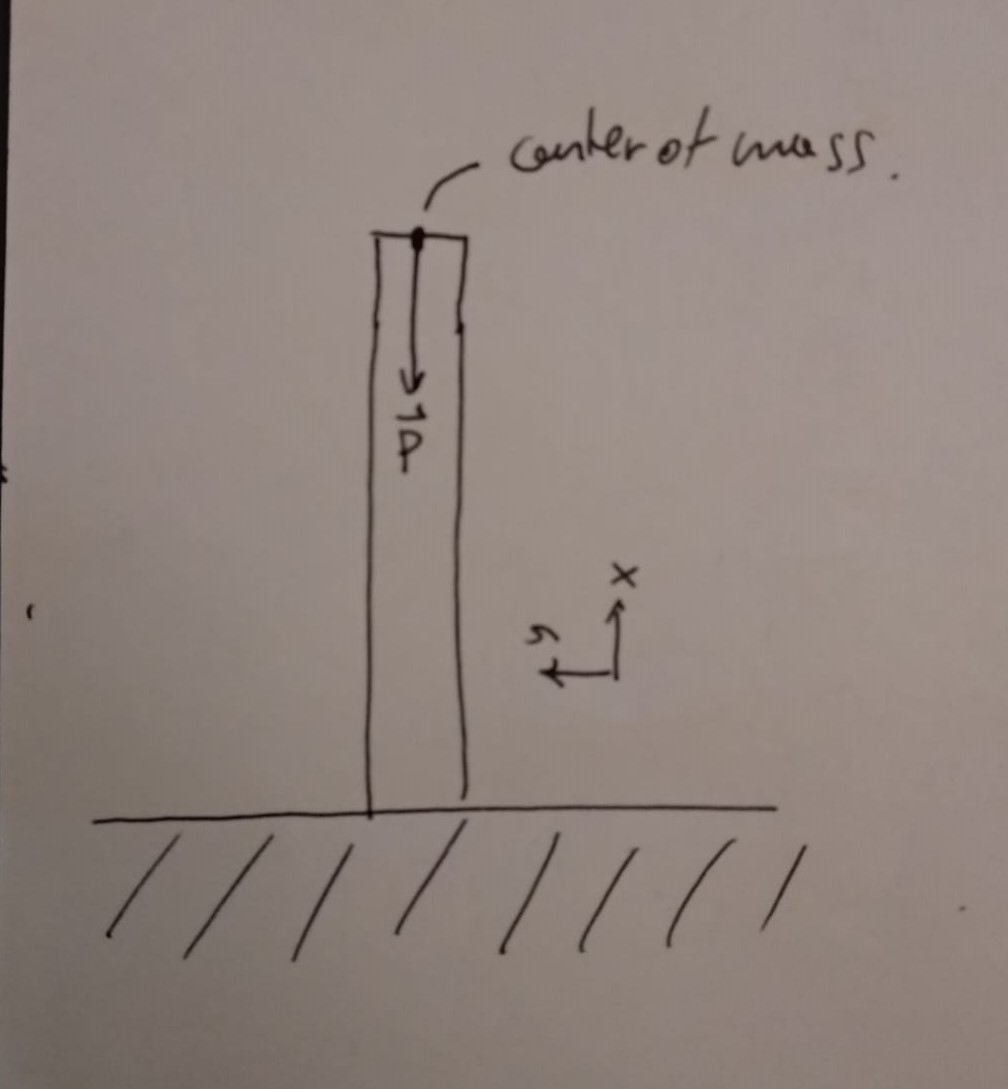
\includegraphics[scale=0.2]{DM3}

Then we have that the equilibrium conditions are given by
$$\begin{cases}
\frac{d\vec{R}}{d\sigma}=\vec{0}\\
\frac{dM}{d\sigma}+\lambda T=0
\end{cases}$$
with the conditions that $\theta(0)=0$, $\theta'(h)=0$, $\vec{R}=cst=\vec{R}(h)=-F_0\vec{e}_x$, $F_0\propto d^2h$. Inextensibility gives $M=B\frac{d\theta}{ds}$, $\lambda=ds/d\sigma=1$. Then from $T=\vec{R}\cdot\vec{n}=F_0\sin(\theta)$ we get the following system
$$\begin{cases}
B\frac{d^2\theta}{ds^2}+F_0\sin\theta=0\\
\theta(0)=0\\
\theta'(h)=0
\end{cases}$$
%Then notice that we can write
%$$B\dot{\theta}\ddot{\theta}+F_0\dot{\theta}\sin\theta=\frac{d}{ds}\bigg(B\frac{\dot{\theta}^2}{2}-F_0\cos\theta\bigg)=0\Rightarrow \frac{\dot{\theta}^2}{2}+\frac{F_0}{B}(1-\cos\theta)=E=cst$$
%The final equaiton we get is 
%$$\frac{\dot{\theta}^2}{2}+\frac{F_0}{B}(1-\cos(\theta))=E$$
Now we can write $B\ddot{\theta}+\frac{F_0}{B}\sin(\theta)=0$ and if  $h$ is big enough, which is the case for the biggest trees in their species, we can linearize the equation thus getting 
$$\ddot{\theta}+\frac{F_0}{B}\theta=0\Rightarrow \theta=A_1\cos(\sqrt{\frac{F_0}{B}}s)+A_2\sin(\sqrt{\frac{F_0}{B}}s)$$then the boundary condition $\theta(0)=0$ tells us that $A_1=0$, whereas the boundary condition $\theta'(h)=0$ tells us that $\sqrt{\frac{F_0}{B}}h=\frac{\pi}{2}+n\pi$. Since we are looking at the first stability bifurcation, we will take $n=0$. Now $B=EI$ where $I$ is the moment of inertia per unit lenght of the tree. We can model the tree as a cylinder of height $h$ and diameter $d$. Then we use that for a cylinder of diameter $d$ the moment of inertia per unit lenght is given by $I=\pi d^4/32$. Therefore $B\propto d^4$; then $F_0$ is the weight of the tree, which is given by $F_0\propto d^2h$. Finally we get that 
$$\frac{d^2h}{d^4}h^2\propto cst\Rightarrow h\propto d^{2/3}.$$


As we can see the problems with this approach are that: we are modeling the tree as a cylinder, which in general is not correct; we are assuming that the tree has constant density; we are neglecting the fact that every tree has a different type of crown; we are not taking into account the fact that some trees might not try to grow as high as possible, maybe due to some climatic or environmental factors (see for example the trees in the desert); we might not have that the total weight is proportional to the weight of the trunk.

\section*{Méthodes d'analyse complexe pour des problèmes d'élasticité bidimensionelle}

\subsection*{1.a)}
If $f$ is a holomorphic function then it is $C^{\infty}$ on all of its domain. 
Then we have that 
\begin{align*}
f'(z)&=\lim_{|h|\to 0}\frac{f(z+h)-f(z)}{h}=\lim_{h_1\to 0,h_2\to 0}\frac{f_1(z_1+h_1,z_2+h_2)-f_1(z_1,z_2)+i[f_2(z_1+h_1,z_2+h_2)-f_2(z_1,z_2)]}{h_1+ih_2}
\end{align*}
now this limit must be valid both when $h_1=0$ and $h_2\to 0 $ and when $h_1\to 0$ and $h_2=0$. From this it follows that 
\begin{align*}
f'(z)&=\frac{\partial f_1(z_1,z_2)}{\partial z_1}+i\frac{\partial f_2(z_1,z_2}{\partial z_1}\\
f'(z)&=-i\frac{\partial f_1(z_1,z_2)}{\partial z_2}+\frac{\partial f_2(z_1,z_2)}{\partial z_2}
\end{align*} from which the Cauchy conditions follow, i.e.
\begin{align*}
\frac{\partial f_1}{\partial z_1}&=\frac{\partial f_2}{\partial z_2}\\
\frac{\partial f_1}{\partial z_2}&=-\frac{\partial f_2}{\partial z_1}
\end{align*}


\subsection*{1.b)}
Since $f_1$ and $f_2$ are $C^2$, then we can exchange the order of derivation, thus getting
$$\Delta f_1=\partial^2_{z_1}f_1+\partial^2_{z_2} f_1=\partial^2_{z_1z_2}f_2+\partial^2_{z_2z_1}(-f_2)=0$$

similarly for $f_2$ we get that 
$$\Delta f_2=\partial^2_{z_1}f_2+\partial^2{z_2}f_2=\partial^2_{z_1z_2}(-f_1)+\partial^2_{z_2z_1}f_1=0$$

\subsection*{2)}
At equilibrium we have that 
$$\phi+\div(\sigma)=0$$
where $$\div(\sigma)=\begin{pmatrix}
\frac{\partial \sigma_{xx}}{\partial x}+\frac{\partial \sigma_{xy}}{\partial y}+\frac{\partial \sigma_{xz}}{\partial z}\\
\frac{\partial \sigma_{yx}}{\partial x}+\frac{\partial \sigma_{yy}}{\partial y}+\frac{\partial \sigma_{yz}}{\partial z}\\
\frac{\partial \sigma_{zx}}{\partial x}+\frac{\partial \sigma_{zy}}{\partial y}+\frac{\partial \sigma_{zz}}{\partial z}
\end{pmatrix}$$Componentwise and using Einstein's notation we can therefore write: $\phi_i+\partial_j(\sigma_{ij})=0$.
Still with Einstein's notation we have that Hooke's law says that 
$$\sigma_{ij}=2\mu \epsilon_{ij}+\lambda \epsilon_{kk}\delta_{ij}$$
Now it follows that 
\begin{align*}
\partial_j\sigma_{ij}=2\mu\partial_j\epsilon_{ij}+\lambda \partial_i\epsilon_{kk}
\end{align*}
and using the fact that $\epsilon_{kk}=\div(\mathbf{u})$ and $\partial_j\epsilon_{ij}=\frac{1}{2}\partial_j(\partial_j u_i+\partial_i u_j)=\frac{1}{2}\partial_{jj}u_i+\frac{1}{2}\partial_j\partial_i u_j=\frac{1}{2}\laplacian u_i+\frac{1}{2}\partial_j\partial_i u_j$
we get that
$\partial_j\sigma_{ij}=2\mu[ \frac{1}{2}\laplacian u_i+\frac{1}{2}\partial_j\partial_i u_j]+\lambda\partial_i\div(\mathbf{u})$. Finally it follows that
\begin{align*}
\phi_i+\mu\laplacian u_i+\mu\partial_j\partial_i u_j +\lambda\partial_i\div(\mathbf{u})=0\Rightarrow \phi+\mu\laplacian \mathbf{u}+(\mu+\lambda)\grad(\div(\mathbf{u}))=0
\end{align*}



\subsection*{3)}
We have that $\mathbf{u}=(0,0,\omega)$,
from which, using the equation found previously, it follows that 
$$\mu\laplacian(\omega)=0\Rightarrow\partial^2_x\omega+\partial^2_y\omega=0$$
where we used the fact that in this case $\div(\mathbf{u})=0$. So $\omega$ is harmonic

%$\epsilon_{xx}=\epsilon_{xy}=\epsilon_{yx}=\epsilon_{yy}=\epsilon_{zz}=0$ and $\epsilon_{zx}=\epsilon_{xz}=\frac{1}{2}\frac{\partial w}{\partial x}$, $\epsilon_{yz}=\epsilon_{zy}=\frac{1}{2}\frac{\partial w}{\partial y}$. 

\subsection*{4)}
We have that 
$$\epsilon=\begin{pmatrix}
0 && 0 && \frac{1}{2}\frac{\partial \omega}{\partial x}\\
0 && 0 && \frac{1}{2}\frac{\partial \omega}{\partial y}\\
\frac{1}{2}\frac{\partial \omega}{\partial x} && \frac{1}{2}\frac{\partial \omega}{\partial y} && 0\\
\end{pmatrix}$$
and from $\sigma_{ij}=2\mu\epsilon_{ij}+\lambda\epsilon_{kk}\delta_{ij}$ we get that 
$$
\sigma=2\mu\begin{pmatrix}
 0 && 0 && \frac{1}{2}\frac{\partial \omega}{\partial x}\\
0 && 0 && \frac{1}{2}\frac{\partial \omega}{\partial y}\\
\frac{1}{2}\frac{\partial \omega}{\partial x} && \frac{1}{2}\frac{\partial \omega}{\partial y} && 0\\
\end{pmatrix}=
\begin{pmatrix}
 0 && 0 && \frac{\partial\text{Im}\Omega}{\partial x}\\
0 && 0 && \frac{\partial\text{Im}\Omega}{\partial y}\\
\frac{\partial\text{Im}\Omega}{\partial x} && \frac{\partial\text{Im}\Omega}{\partial y} && 0\\
\end{pmatrix}$$
Finally we have that $\sigma_{yz}+i\sigma_{xz}=\frac{\partial\text{Im}\Omega}{\partial y}+i\frac{\partial\text{Im}\Omega}{\partial x}=\frac{\partial\text{Re}\Omega}{\partial x}+i\frac{\partial\text{Im}\Omega}{\partial x}=\Omega'$.

\subsection*{5)}
From $\log(z)=\ln(|z|)+i\arg(z)$ we get that $\Omega(z)=-i\ln(|z|)/2\pi+\arg(z)/2\pi$, which implies that the displacement field has its $z$ component $\omega$ given by $\mu\omega(x,y)=-\ln(\sqrt{x^2+y^2})/2\pi$. Then it follows that $\mu\partial_x\omega=-\frac{1}{2\pi}\frac{x}{x^2+y^2}$ and $\mu\partial_y\omega=-\frac{1}{2\pi}\frac{y}{x^2+y^2}$, and finally
$$\sigma=-\frac{1}{2\pi}\frac{1}{x^2+y^2}\begin{pmatrix}
0 && 0 && x\\
0 && 0 && y\\
x && y && 0
\end{pmatrix}$$
If we look directly at the displacement field we can suddenly see that we are in a situation where a generical continuous medium under this field of contraint will be bended downwards by a quantity which increases as we go further from the origin for $x^2+y^2>1$, whereas it will be bended upwards for $x^2+y^2<1$. A picture that represents the profile of such a deformed medium is the following:\\

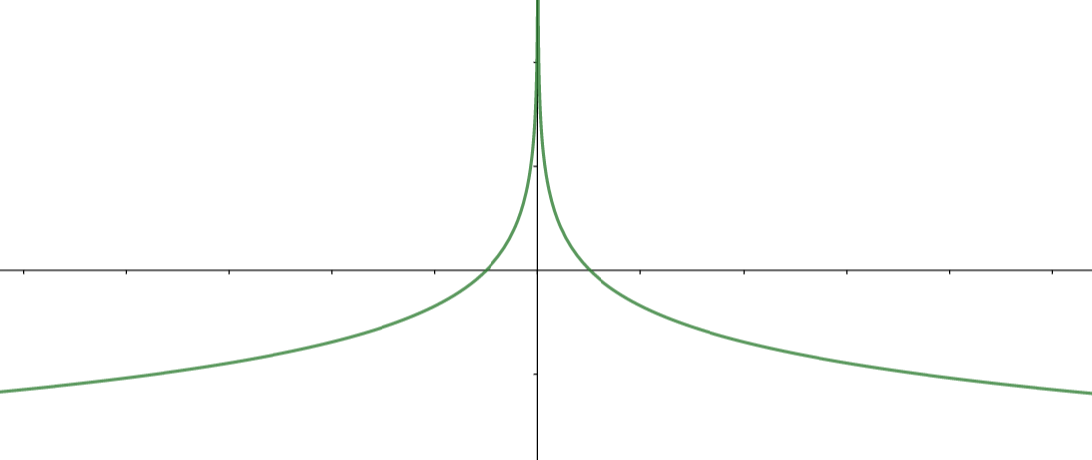
\includegraphics[scale=0.5]{DM1}


In particular, since the displacement field only depends on the distance from the origin, no matter how we take a plane containing the $z-$axis, the profile will always be the same (as above). This can be thought as a situation in which we take for example a flat and square elastic material (like the material of a balloon) and we pull it vertically from the center: it will then assume a form which is similar to the picture above.

\subsection*{6.a)}
With $z$ we mean the complex number $x+iy$, with $\zeta$ we mean the $\vec{e}_z$ component of a general vector in $\mathbb{R}^3$.
At infinity we have that  $$\sigma_{\infty}=\begin{pmatrix}
0 && 0 && 0\\
0 && 0 && S\\
0 && S && 0
\end{pmatrix}$$
hence the behaviour of $\Omega$ should be such that when $|z|$ goes to infinity, then $\partial_y\text{Im}\Omega\to S$ and $\partial_x\text{Im}\Omega\to 0$, which by the Cauchy conditions also imply that 
$\partial_x\text{Re}\Omega\to S$ and $\partial_y\text{Re}\Omega\to 0$.
The constraint force at any point on the planes $y=\pm y_l$ is given by 
$$T(x,y)_{\pm}=\sigma_{\infty}\cdot \begin{pmatrix}
0\\
\pm1\\
0
\end{pmatrix}=\begin{pmatrix}
0\\
0\\
\pm S
\end{pmatrix}$$hence we have the following schéma

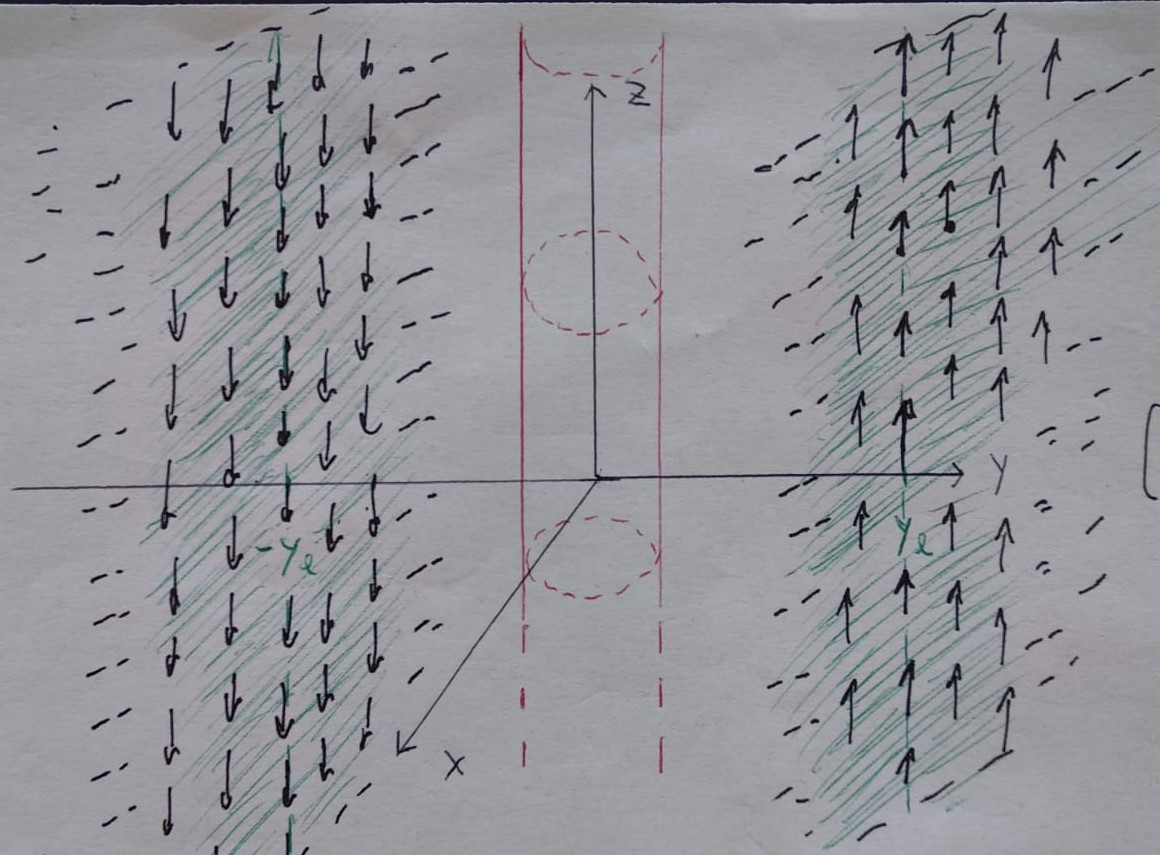
\includegraphics[scale=0.3]{DM2}

where the green parts represent the planes $\pm y_l$, where at each point  of these there is applied a force $(0,0,\pm S)$ which comes from the tensor of constraints that is applied.


\subsection*{6.b)}
If we call $z=x+iy$, then we have that $\Omega=S(z-R^2/z)=S\bigg(x-\frac{R^2x}{x^2+y^2}+i\frac{x^2y+R^2y+y^3}{x^2+y^2}\bigg)$ from which it follows that $\omega(x,y)=\frac{S}{\mu}\frac{x^2y+R^2y+y^3}{x^2+y^2}$. The displacement field is given by $\mathbf{u}=(0,0,\omega)$. Finally we have that 
$$\frac{\partial\text{Im}\Omega}{\partial x}=-S\frac{2R^2xy}{(x^2+y^2)^2}$$
$$\frac{\partial\text{Im}\Omega}{\partial y}=S\bigg(\frac{R^2(x^2-y^2)}{(x^2+y^2)^2}+1\bigg)$$
so that 
$$\sigma=
\frac{S}{(x^2+y^2)^2}
\begin{pmatrix}
0 && 0 && -2R^2xy\\
0 && 0 && R^2(x^2-y^2)+(x^2+y^2)^2\\
-2R^2xy && R^2(x^2-y^2)+(x^2+y^2)^2 && 0
\end{pmatrix}
$$
We have the following behaviors:
\begin{itemize}
\item for $\partial_x\text{Im}\Omega=-S\frac{2R^2xy}{(x^2+y^2)^2}$:

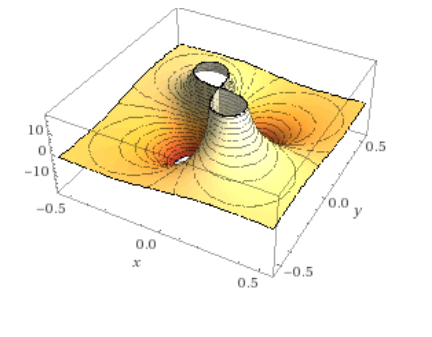
\includegraphics[scale=0.6]{fm1}
\item for $\partial_y\text{Im}\Omega=\bigg(S\frac{R^2(x^2-y^2)}{(x^2+y^2)^2}+S\bigg)$:
\\
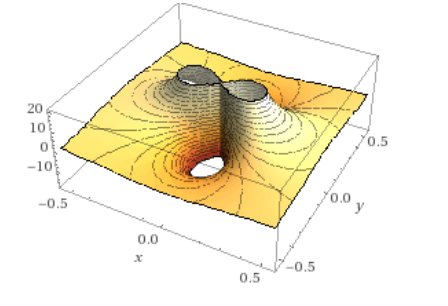
\includegraphics[scale=0.6]{fm2}

\end{itemize}


\subsection*{6.c)}
On the interior boundary we have that
any point can be expressed as $x=R\cos(\theta)$ and $y=R\sin(\theta)$ so that we get
\begin{align*}
\sigma_{xz}&=-S\sin(2\theta)\\
\sigma_{yz}&=S(\cos(2\theta)+1)
\end{align*}

Then we verify that for any unit vector pointing out from the interior surface of the cylinder we have:
$$\begin{pmatrix}
0 && 0 && \sigma_{xz}\\
0 && 0 && \sigma_{yz}\\
\sigma_{xz} && \sigma_{yz} && 0
\end{pmatrix}\cdot 
\begin{pmatrix}
R\cos(\theta)\\
R\sin(\theta)\\
0
\end{pmatrix}=SR\begin{pmatrix}
0 \\
0\\
-\sin(2\theta)\cos(\theta)+\sin(\theta)(\cos(2\theta)+1)
\end{pmatrix}=\vec{0}
$$
since $-\sin(2\theta)\cos(\theta)+\sin(\theta)(\cos(2\theta)+1)=-2\sin(\theta)\cos(\theta)^2+\sin(\theta)(1-2\sin(\theta)^2)+\sin(\theta)=0$.
So we see that the funciton $\Omega$ satisfies indeed the boundary conditions on the interior border. 
Moreover we have that at infinity $\Omega$ is such that 
$$\partial_{x}\text{Im}\Omega=-2\frac{SR^2xy}{(x^2+y^2)^2}\to 0$$
$$\partial_y\text{Im}\Omega=\frac{SR^2(x^2-y^2)}{(x^2+y^2)^2}+S\to S$$
hence we see that this $\Omega$ satisfies the right boundary conditions both internally and externally, which makes it a good candidate in order to study the tensor of constraints for the situation where we have a cylindrical hole parallel to the $z-$axis and where we apply the constraint $\sigma_{xz}=0$, $\sigma_{yz}=S$ at infinity on the planes $y=\pm y_l$.


\subsection*{7.a)}
We have that 
\begin{align*}
\Gamma(z_0)=\frac{a+b}{2}z_0+\frac{a-b}{2z_0}=x_0\frac{a(|z_0|^2+1)+b(|z_0|^2-1)}{2|z_0|^2}+iy_0\frac{a(|z_0|^2-1)+b(|z_0|^2+1)}{2|z_0|^2}
\end{align*}
which implies that 
$$x:=\text{Re}\Gamma=x_0\frac{a(x_0^2+y_0^2+1)+b(x_0^2+y_0^2-1)}{2(x_0^2+y_0^2)}$$
$$y:=\text{Im}\Gamma=y_0\frac{a(x_0^2+y_0^2-1)+b(x_0^2+y_0^2+1)}{2(x_0^2+y_0^2)}$$

Now we want to see where circles of radius $r$ are mapped by $\Gamma$: suppose we consider the circle of radius $r$, i.e. the set of points satisfying $x_0^2+y_0^2=r^2$, then we get that
$$\begin{cases}
x=x_0\big(\frac{a+b}{2}+\frac{a-b}{2r^2}\big)\\
y=y_0\big(\frac{a+b}{2}-\frac{a-b}{2r^2}\big)
\end{cases}\Rightarrow \frac{x^2}{\big(\frac{a+b}{2}+\frac{a-b}{2r^2}\big)^2}+\frac{y^2}{\big(\frac{a+b}{2}-\frac{a-b}{2r^2}\big)^2}=r^2$$
hence the image of a circle of radius $r$ is an ellipse with semi-major and semi-minor axes given respectively by $r\frac{a+b}{2}+\frac{a-b}{2r}$ and $r\frac{a+b}{2}-\frac{a-b}{2r}$. Since the circle of radius $1$ has been excluded from the domain, it follows that the ellipse of semi-major and semi-minor axes given by $a,b$ is not mapped by any circle. In order to conlude that the image of $\Gamma$ is the complex plane without the area enclosed by the ellipse of axes $a,b$ we need to show that all the circles with radius $r>1$ are mapped by $\Gamma$ to ellipses of semi-major and semi-minor axes that are respectively bigger than $a$ and $b$.
In particular consider a generical ellipse of the type found above, $\frac{x^2}{\big(r\frac{a+b}{2}+\frac{a-b}{2r}\big)^2}+\frac{y^2}{\big(r\frac{a+b}{2}-\frac{a-b}{2r}\big)^2}=1$, mapped by $\Gamma$ from a circle of radius $r>1$; then we have that 
\begin{align*}
&r\frac{a+b}{2}+\frac{a-b}{2r}>a\\
\Leftrightarrow & r^2(a+b)-2ar+(a-b)>0\\
\Leftrightarrow & (r-1)(r-\frac{a-b}{a+b})>0\\
\Leftrightarrow &\text{True, since }r>1
\end{align*}

and \begin{align*}
&r\frac{a+b}{2}-\frac{a-b}{2r}>b\\
\Leftrightarrow &r^2(a+b)-2rb-(a-b)>0\\
\Leftrightarrow &(r-1)(r-\frac{b-a}{a+b})>0\\
\Leftrightarrow &\text{True, since }r>1
\end{align*}.Hence, since the domain of $\Gamma$ was the complex plane without the disk of radius $1$, we have that the area enclosed by the ellipse of axes $a,b$ does not belong to the image of $\Gamma$. It remains to prove that all the rest of the complex plane belongs to the image of $\Gamma$. Proving this is equivalent  to showing that for any point that doesn't belong to the area enclosed by the ellipse of axes $a,b$ there is a radius $r>1$ such that the ellipse $\frac{x^2}{\big(r\frac{a+b}{2}+\frac{a-b}{2r}\big)^2}+\frac{y^2}{\big(r\frac{a+b}{2}-\frac{a-b}{2r}\big)^2}=1$ passes through that point. In a simpler way we can notice that both $r\frac{a+b}{2}+\frac{a-b}{2r}$ and $r\frac{a+b}{2}-\frac{a-b}{2r}$ are continuous increasing functions for $r>1$; moreover we have that they both tend to infinity as $r\to\infty$. This means that as we let $r\to\infty$, the ellipses generated by $\Gamma$ from the circles of radius $r$ will pass on the entirety of the complex plane (not including the zone included in the ellipse of axes $a,b$).

\subsection*{7.b/c)}

We have that, by the chain rule:
$$(\Omega\circ\Gamma)'=(\Omega'\circ\Gamma)\cdot \Gamma'$$then we know by question 6 that $\Omega'(z)=S\big(1+\frac{R^2}{z^2}\big)$. 
Hence if we call $z=\Gamma(z_0)$ then we have that 
$$(\Omega\circ \Gamma)'(z_0)=(\Omega'\circ \Gamma)(z_0)\cdot\Gamma'(z_0)\Rightarrow (\Omega\circ\Gamma)'(z_0)=S\bigg(1+\frac{R^2}{z^2}\bigg)\Gamma'(z_0)$$

%We know $\Gamma(z_0)$
%
%
%
%The field of constraint is given by $\sigma_{yz}+i\sigma_{xz}=\Omega'$, thanks to the question 4.
%Now we have that 
%$$\frac{\partial \Omega(\Gamma(z_0))}{\partial z_0}=\frac{\partial \Omega(\Gamma(z_0))}{\partial \Gamma(z_0)}\frac{\partial\Gamma(z_0)}{\partial z_0}=\frac{\partial\Omega(z)}{\partial z}\frac{\partial \Gamma(z_0)}{\partial z_0}\Rightarrow \Omega'(z)=\frac{\partial\Omega(\Gamma(z_0))}{\partial z_0}\bigg(\frac{\partial \Gamma(z_0)}{\partial z_0}\bigg)^{-1}$$ 
Now, from $\Gamma(z_0)=\frac{a+b}{2}z_0+\frac{a-b}{2z_0}$ it follows that 
$$\frac{d\Gamma(z_0)}{d z_0}=\frac{a+b}{2}-\frac{a-b}{2z_0^2}$$
%Then, using $R=1$ since we are considering the radius of the unit circle, we get:
%$$\Omega(\Gamma(z_0))=S(\Gamma(z_0)-1/\Gamma(z_0))=S\bigg(\frac{a+b}{2}z_0+\frac{a-b}{2z_0}-\frac{1}{\frac{a+b}{2}z_0+\frac{a-b}{2z_0}}\bigg)=S\bigg(\frac{a+b}{2}z_0+\frac{a-b}{2z_0}-\frac{2z_0}{(a+b)z_0^2+(a-b)}\bigg)$$
%then it follows that 
%$$\partial_{z_0}\Omega(\Gamma(z_0))=S\bigg(\frac{a+b}{2}-\frac{a-b}{2z_0^2}+2\frac{a(z^2-1)+b(z^2+1)}{(a(z^2+1)+b(z^2-1))^2}\bigg)$$
So, recalling that now $R=1$, finally we get that the new constraint field is given by
$$\sigma_{yz}+i\sigma_{xz}=S\bigg(1+\frac{1}{(\frac{a+b}{2})^2z_0^2+(\frac{a-b}{2z_0})^2+\frac{(a+b)(a-b)}{2}}\bigg)\bigg(\frac{a+b}{2}-\frac{a-b}{2z_0^2}\bigg)$$

For $z_0=1$ we simply have that 
$$\sigma_{yz}+i\sigma_{xz}=S\bigg(b+\frac{b}{a^2}\bigg)$$
we see that at $z_0=1$ we have $\sigma_{yz}=S\big(b+\frac{b}{a^2}\big)$ and $\sigma_{xz}=0$. In the case $a=b=1$ we see that we get back the boundary conditions of the unit circle on the interior surface at the point $z_0=1$.
\subsection*{7.d)}

The interest of this approach lies on the fact that we can directly find the field of constraints for the ellipse from the simple case of the circle, without having to look for a specfic $\Omega$ that would give a solution for the ellipse. This suggests the fact that since we found a good $\Omega$ for the case of the circle, then we could find the right $\Omega_{new}$ for any type of geometrical figure for which we can find a conformal map that maps the unit circle in the new geoemtrical figure.
























\end{document}